\documentclass{elektr}
\usepackage{hyperref}
\hypersetup{
colorlinks=true,
urlcolor=black,
citecolor=blue}
\usepackage[all]{xy,xypic}
\usepackage{amsfonts,amssymb,amsmath,amsgen,amsopn,amsbsy,theorem,graphicx,epsfig}
\usepackage{eufrak,amscd,bezier,latexsym,mathrsfs,eurosym,enumerate}
\usepackage[utf8]{inputenc}
\usepackage[english]{babel}
\usepackage{cleveref,multirow}
\usepackage[dvipsnames]{xcolor}
\usepackage[pagewise]{lineno}
\usepackage{float}
\usepackage{subcaption}
% -------- Clean version: revision markers stripped --------
% \yh{...} is defined as a transparent pass-through so all reviewer-driven
% edits render as normal body text (no colour, no highlight). Use this
% file for camera-ready / final submission after the revisions are
% accepted; the highlighted sibling (main_highlighted.tex) keeps the same
% content but shows those same edits with a yellow background.
\newcommand{\yh}[1]{#1}
\linenumbers

\yil{}
\vol{}
\fpage{}
\lpage{}
\doi{}

\title{
	Shoulder-Based Myoelectric Control for Prosthetic Hand Operation in Transhumeral Amputees Using a Hybrid Deep Learning Model }
\author[KAUR et al.]{
	\textbf{Amanpreet KAUR$^{1}$~, Hemanshu MANDHANA$^{2,*}$, Gazal ARORA$^{3,*}$, Arnav JAIN$^{4,*}$}\\

	$^{1}$Electronics and Communication Engineering Department, Faculty, TIET, Patiala, India (aman.preet@thapar.edu)\\ 	\url{https://orcid.org/0000-0002-8714-9507} \\
	$^{2,3,4}$Computer Science and Engineering Department, Student, TIET, Patiala, India\\
	$^{*}$These authors contributed equally to this work.\\

	\rec{...}
	\acc{...}
	\finv{...}
}

\input{elksty.tex}

\setcounter{page}{1}
\begin{document}

\maketitle

\begin{abstract} Surface electromyography (sEMG) is becoming increasingly important for responsive, intuitive control in prosthetic technology. While extensively studies is focused on decoding hand and finger movements, but shoulder movement control has received less attention.  This is particularly important for  transhumeral amputees who lack distal muscle signals, To address this gap, the present study  explore the use of these signals for prosthetic hand control, this study performs an initial analysis of sEMG patterns from key shoulder muscles (Pectoralis Major, Trapezius, and Teres Major) in eight right-hand transhumeral amputees.This work presents a hybrid deep learning architecture that leverages convolutional neural networks (CNNs) for spatial feature extraction and long short-term memory (LSTM) networks for temporal sequence modeling, followed by a classical meta-classifier for robust classification of shoulder movements, including elevation, protraction, and retraction. The suggested hybrid model has a sensitivity of 97.32\%, an F1-score of 97.28\%, and an accuracy of 97.31\%. The findings show that combining CNN and LSTM architectures reliably and effectively categorizes shoulder movements of transhumeral amputees. This work advances the development of myoelectric prosthetic systems for transhumeral amputees by introducing a shoulder-based control approach enabling three essential movements: hand opening,closing, and elbow motion.
 
 
 \newcommand{\keywords}[1]{\textbf{Keywords:} #1}
\keywords{Transhumeral Amputees, surface Electromyog­ raphy, Deep Learning, Prosthetic Control,Time-Series Classifica­tion,CNN-LSTM}
\end{abstract}

\section{Introduction}
\label{Int}

Disability issues have a significant impact on people's living standards worldwide. People who have had their upper limbs amputated have a lot of trouble with their everyday lives and their quality of life. Prosthetic devices have been developed to help amputees regain some functionality \cite{prakash2020force}, \cite{desplenter2020rehabilitative}. But there are still many challenges to overcome to improve their usefulness and efficacy. For upper-limb amputees, shoulder movements often serve as a compensatory mechanism for the development of responsive, intuitive prosthetic devices. While most research has focused on categorizing specific motions by decoding finger and hand movements from surface electromyography (sEMG) electrodes placed on the body, some studies have focused on shoulder movements in transhumeral amputees. These individuals often have difficulty controlling their prostheses due to a lack of distal muscle activity. Extracting these motions from EMG signals is a considerable challenge.\\
\indent
Currently, mechanisms supporting two degrees of freedom are relatively simple and widely employed \cite{chaobankoh2024classification}. Sensors need to be carefully positioned in a well-designed location to achieve more DOF \cite{jarrasse2016classification}. Usually, myoelectric upper-limb prostheses use two upper extremity actuators to control one degree of freedom (DoF)  \cite{thomson2025myoelectric}. Myoelectric prostheses with multiple degrees of freedom can be better controlled for transhumeral amputees by implanting a sensor in their shoulder \cite{chaobankoh2024classification},\cite{jarrasse2016classification}. Once sEMG signals are captured via strategically placed sensors, accurately interpreting them becomes critical for prosthetic control. For this purpose, various classification techniques have been employed to decode the intended movements. As an effective means to classify sEMG patterns\cite{li2017motion,xie2015comparative,thermalBreastXAI},several different classifier methods include artificial neural networks (ANNs), support vector machines (SVM) \cite {singh2020comparative}, fuzzy logic (FL), genetic algorithms (GA), linear discriminant analysis (LDA), naive Bayes (NB), K-Nearest Neighbours (KNN), AdaBoost, Random Forests (RF) and others \cite{seyidbayli2020comparison}. Acquiring sEMG signals from muscles to categorize specific shoulder movements is a considerable challenge \cite{rani2023surface}. The stochastic nature and high variability of sEMG signals make it difficult for different classifiers to handle this information; thus, the choice of an appropriate classifier is critical\cite{zhang2024improving}. To address this, Trigili et al;\cite{trigili2019detection} developed a machine learning-based algorithm to detect and classify movements of the upper extremities, using pattern recognition. Furthermore, \yh{recent works published between 2023 and 2026 have significantly extended EMG-based classification research, including deep-learning pipelines for real-time gesture decoding} \cite{ref2024_en17112539,ref2024_electronics13173552}\yh{, hybrid CNN--LSTM frameworks for prosthetic control} \cite{ref2025_cmes065098}\yh{, and energy-efficient EMG signal processing systems} \cite{ref2024_en17215412}\yh{. These recent contributions complement the earlier literature, yet continue to focus predominantly on distal-muscle recordings; the shoulder-region emphasis of the present study addresses a comparatively under-explored gap.}\\
\indent By increasing the degrees of freedom (DOFs) of an existing portable upper-limb exoskeleton, this author\cite{truong2024design} seeks to improve its design without sacrificing performance by keeping the structure lightweight and uncomplicated. The suggested system will include four DOFs in total: three at the shoulder joint to facilitate multidirectional movement and one at the elbow joint for flexion and extension. Wearable robotic exoskeleton with EMC control for upper arm rehabilitation that uses Long Short-Term Memory (LSTM) networks to control motion adaptively \cite{samarakoon2025long}. Some authors used data directly obtained from transhumeral amputees \cite {kimizuka2020shoulder} to enhance the clinical significance of the control system. A study \cite{gaudet2018classification} where transhumeral amputees' residual limbs were surrounded by six evenly spaced sEMG channels. The feasibility of using residual shoulder muscle activity for upper-limb prosthesis control was demonstrated by the authors' use of a multilayer perception (MLP) trained with backpropagation, achieving an average classification accuracy of 81.1\%\\
\indent Hurtado et al\cite{hurtado2024movements} developed a classification system for elbow movements in elbow dis-articulation. Five elbow movements were recorded over different time intervals. A comprehensive feature set, such as mean absolute value (MAY), zero crossings (ZC), signal sign changes (SSC), etc., was extracted. Six different classifiers, such as Random Forest (RF), Linear Discriminant Analysis (LDA), Quadratic Discriminant Analysis (QDA), k-Nearest Neighbors (KNN), Support Vector Machine (SVM), and Multilayer Perceptron (MLP), were tested to classify the movements, with hyper parameters optimized using cross-validation. Among the classifiers, the random forest (RF) model achieved the highest accuracy of 74.85\% ± 6.28\%, outperforming all other models. However, because the shoulder region is where the majority of upper-limb muscle activity originates in upper-limb amputees, sensor placement presents a significant challenge. Since the electromyography signals from the shoulder muscles must accurately depict the intended movements of the missing limb, it is crucial but challenging to capture and interpret these signals \cite{berjis2025selecting,reilly2020computational}.\\
\indent Despite extensive research on decoding upper-limb movements using EMG signals, most available studies emphasize the distal muscles of the forearm and wrist. Comparatively fewer efforts have been made to explore EMG activity originating from the shoulder region, which plays a central role in motion control for transhumeral amputees. This observation forms the key motivation       of the present study. \\
The present work makes several notable contributions.\\
•	It focuses on the analysis of EMG signals obtained from the Pectoralis Major, Trapezius, and Teres Major muscles, a relatively unexplored source of control information for transhumeral amputees who lack distal muscle activity.\\
•	Convolutional and recurrent layers are integrated into a combined deep learning framework to take advantage of the EMG signals' temporal and spatial properties.\\
•	The proposed model demonstrates a substantial improvement in recognition performance, achieving sensitivity, F1-score, and accuracy values of 97.32\%, 97.28\%, and 97.31\%, respectively, when compared with individual CNN or LSTM models.\\
•	These results highlight the potential of shoulder-based EMG decoding as a basis for the upcoming generation of wearable, real-time prosthetic control systems that can facilitate multi-joint movement that is both natural and adaptive.\\
•	Three crucial prosthetic functions—hand opening, hand closing, and elbow motion—are mapped to the decoded shoulder movements. This creates a workable control plan for myoelectric prosthetic systems for transhumeral amputees.\\
•	This work offers a clinically relevant proof-of-concept for shoulder-driven prosthetic control by validating the method on actual amputee data, advancing the development of more user-friendly and accessible myoelectric systems.
\section{Materials and Methods}
This study proposes a novel and robust methodology for classifying muscle activity using sEMG signals, specifically designed to overcome the challenges associated with inter-subject variability.  The proposed  framework is built in the form of a multi-step processing pipeline covering data capture, quality-dependent sampling, window-based temporal segmentation, rich feature extraction, and final classification. As illustrated in Figure~\ref{fig:emg classification}, each module of the framework is described in detail in subsequent sections to support clarity and reproducibility.

The selected feature set is diligently designed to integrate both time-domain and frequency-domain information. This wide-ranging representation allows for greater discriminative power among input features, and thus the classifier can differentiate between fine differences in muscle activation related to various hand gestures. Through the use of this multi-aspect framework, the system is designed for high robust classification performance and generalization across subjects..
\subsection{Participants and Data Acquisition}
To evaluate the practical effectiveness of the proposed method, experiments were conducted using sEMG data collected from eight transhumeral amputees. The participants were aged between 30 and 50~years, weighed between 70 and 110~kg, and had a time since amputation ranging from 10 to 20~years\cite{amanpreet2019machine} Informed consent was obtained from all participants prior to their inclusion in the study.
sEMG signals were recorded from three shoulder muscles---Teres Major, Trapezius, and Pectoralis Major during three different movements: elevation, protraction, and retraction.
\cite{amanpreet2019machine}\cite{kaur2022stacking}. 

	\begin{figure}
	\centering
	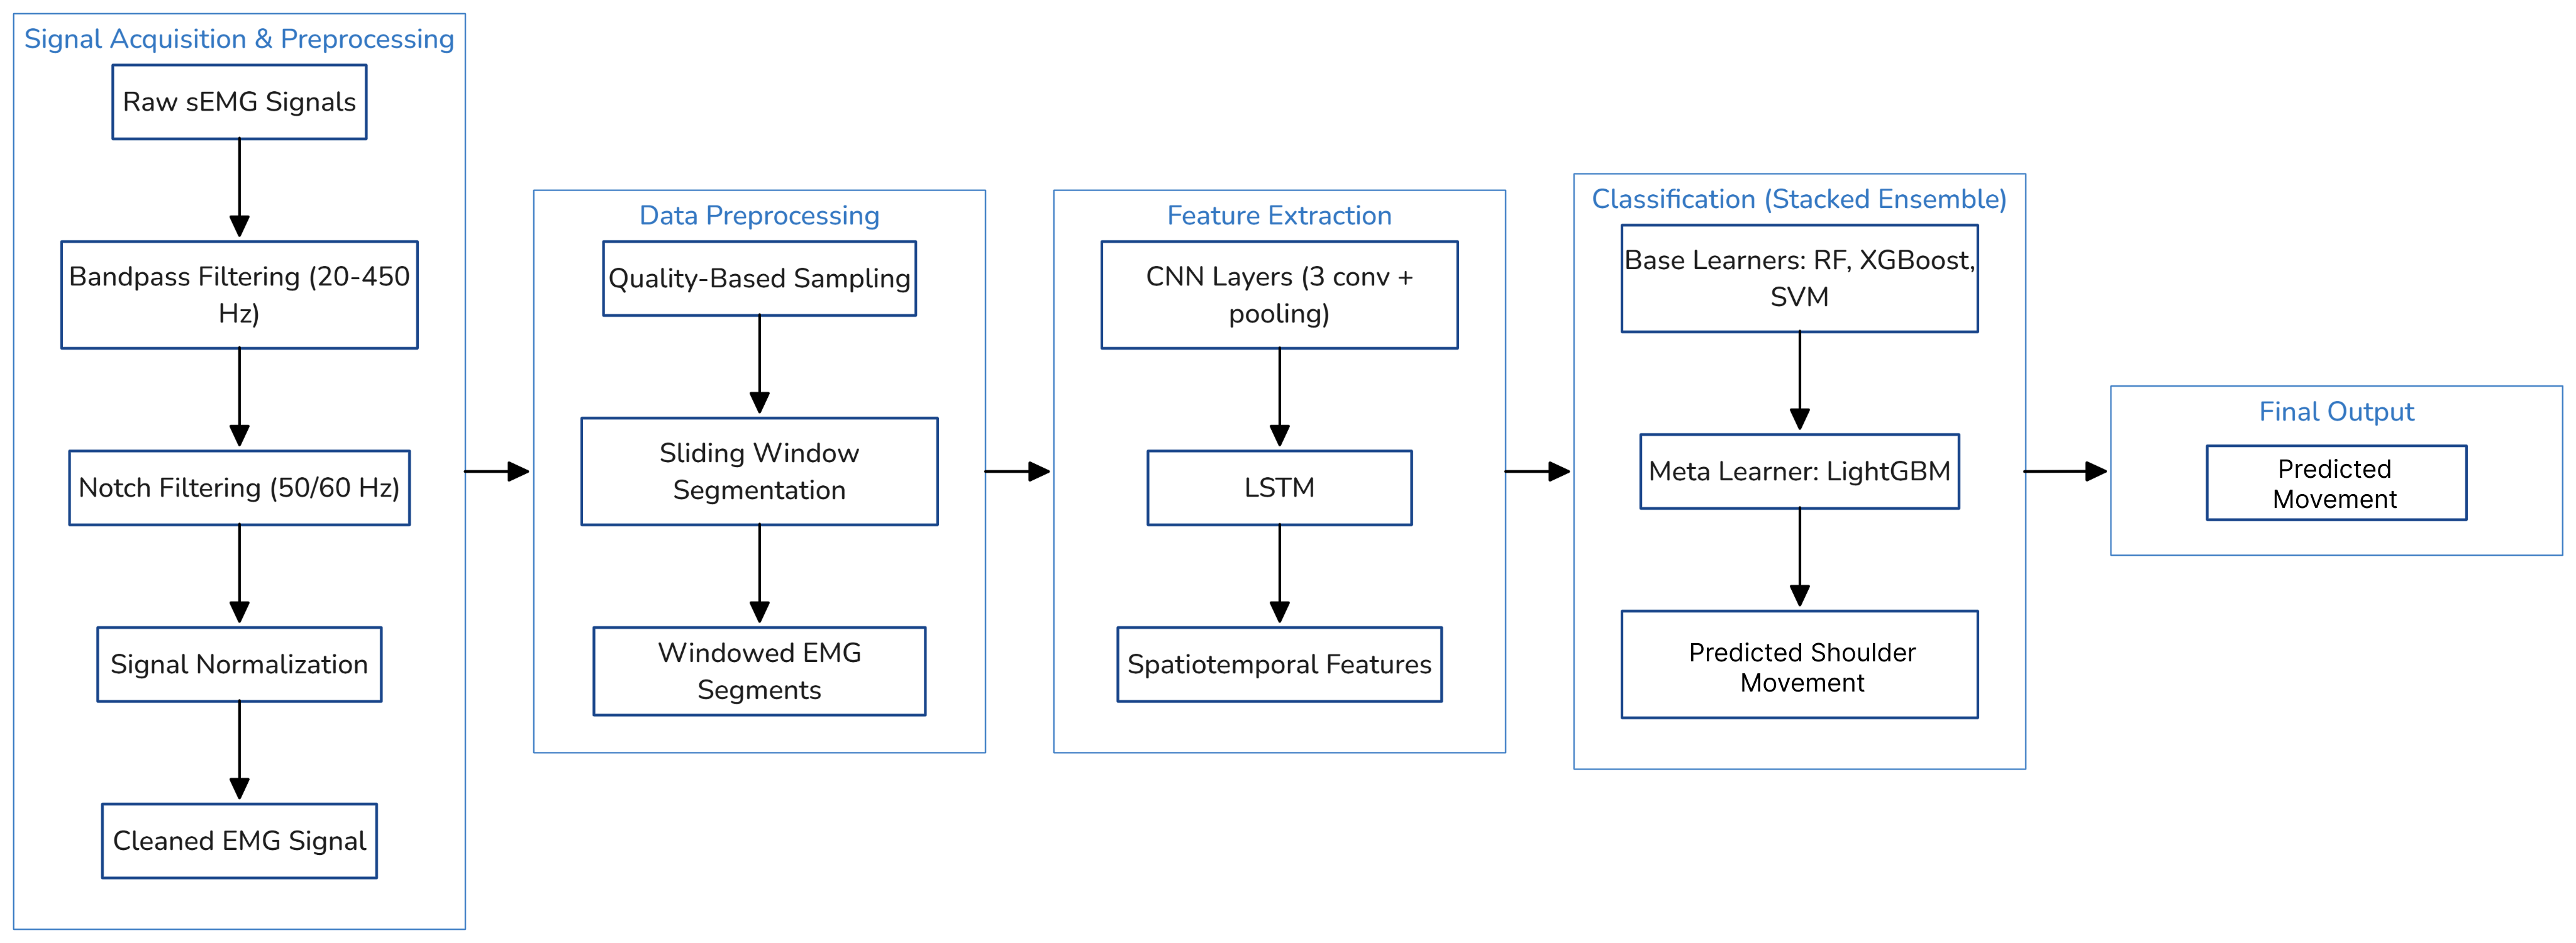
\includegraphics[width=0.83\linewidth]{research.png}
	\caption{The proposed EMG classification pipeline, comprising preprocessing, segmentation, deep feature extraction, and ensemble-based classification}
	\label{fig:emg classification}
\end{figure}
\subsection{Signal Preprocessing}
The signal channels recorded using surface electrodes were sensitive to noise and subject-specific variability, including differences in muscle physiology. Preprocessing was essential to enhance the quality and consistency of the EMG signals. For acquiring sEMG signal, NeXus-10~ Mark II TMS International BV, a multi-channel physiological monitoring and feedback platform system, has been used for live data. In the sEMG system, the notch filter is used to suppress the 50~Hz main power interference. The sEMG system has a gain factor of 19.5 and CMRR $\geq 100\,\mathrm{dB}$. The analog-to-digital resolution is 12.2~nV/bit. The four-channel system is used to acquire data for two degrees of freedom. The raw sEMG sample rate is 2048 samples per second. Each sample has a 24-bit resolution. The signal is filtered out by the fourth-order IIR bandpass Butterworth filter with a frequency range between 20-500~Hz \cite{amanpreet2019machine,kaur2022stacking}. 

\subsection{Shoulder Movement Protocol and Angle Measurement}
Participants were instructed to perform controlled shoulder elevation, protraction, and retraction movements. The horizontal alignment and angle of the shoulder were monitored using motion analysis software as participants performed the movement task Figure~\ref{fig:shoulder_movement}. The GaitON motion analysis tool, which uses visual markers and calibrated video analysis to precisely track postural and joint angles, was used to obtain the shoulder alignment measurements. The monitoring was conducted based on the angle to ensure the task was executed correctly.
\begin{figure}
	\centering
	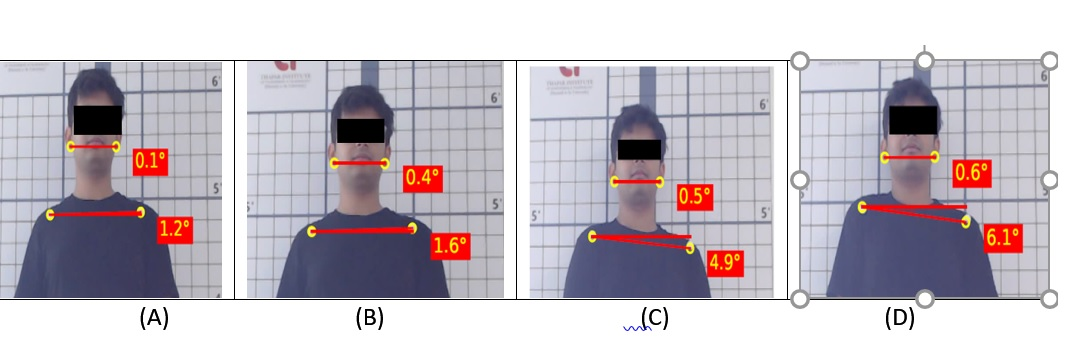
\includegraphics[width=\linewidth]{1234.jpg}
	\caption{Quantitative shoulder angle measurement during controlled shoulder movement tasks. 
		(a) Neutral alignment, (b) mild deviation, (c) moderate left shoulder depression, and 
		(d) increased left shoulder depression.}
	\label{fig:shoulder_movement}
\end{figure}
Figure~\ref{fig:shoulder_movement} presents quantitative measurements of shoulder alignment corresponding to the performed shoulder movements. Panel~(a) represents the initial neutral position prior to movement, showing minimal angular deviation of the head ($-0.1^\circ$) and right shoulder ($+1.2^\circ$).

Panel~(b) illustrates the initial displacement associated with controlled movement onset. The head and right shoulder remain nearly horizontally aligned, with angular deviations of $-0.4^\circ$ and $+1.6^\circ$, respectively, indicating minimal deviation from the neutral posture.

Panel~(c) demonstrates progressive left shoulder depression, where the angular deviations of the head and right shoulder are $-0.5^\circ$ and $-4.9^\circ$, respectively.

Finally, Panel~(d) corresponds to a greater shoulder movement amplitude, with angular deviations of $+0.6^\circ$ for the head and $-6.1^\circ$ for the right shoulder.

These angular variations confirm the controlled execution of shoulder elevation, protraction, and retraction tasks used for sEMG signal labeling.

\subsection{Windowing Strategy }
	To convert real-time sEMG signals into an appropriate learning input format, a sliding window method was adopted, as shown in Figure ~\ref{fig:Sampled EMG signal}. The visualization has been divided into three parts showing  the data after sampling  and the windowing process of sEMG signal. 
	
			
		\begin{figure}
			\centering
			
			\begin{subfigure}[!b]{0.48\columnwidth}
				\centering
				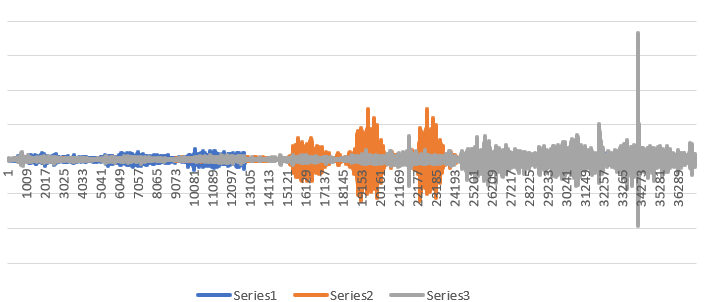
\includegraphics[width=\linewidth,height=4cm,keepaspectratio]{Screenshot 2025-04-24 215712.png}
				\caption{Sampled EMG signal}
			\end{subfigure}
			\hfill
			\begin{subfigure}[!b]{0.48\columnwidth}
				\centering
				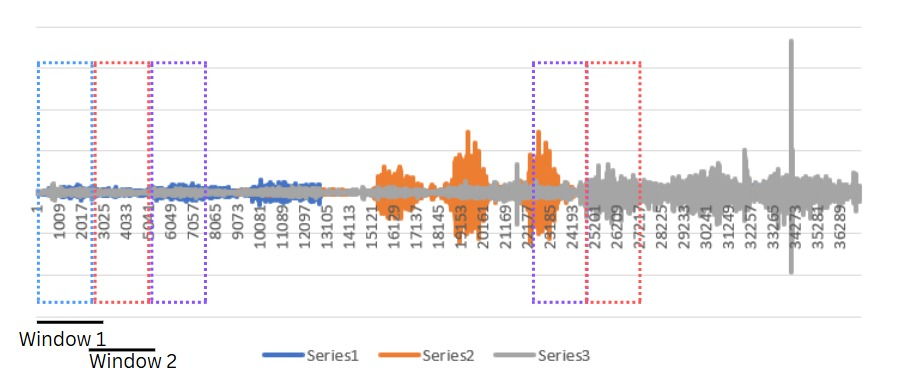
\includegraphics[width=\linewidth,height=4cm,keepaspectratio]{Screenshot 2025-04-24 231131.png}
				\caption{Windowed EMG signal}
			\end{subfigure}
			
			\caption{EMG signal visualization: (a) sampled signal, (b) segmented signal}
			\label{fig:Sampled EMG signal}
		\end{figure}
		
		\begin{itemize}
			\item $l$ denotes the convolutional layer index,
			\item $k$ is the filter index,
			\item $C = 3$ is the number of channels,
			\item $K = 3$ is the kernel size,
			\item $\sigma(\cdot)$ is the ReLU activation,
			\item $x^{(l-1)}_c$ is the input feature from channel $c$ at layer $l-1$,
			\item $w^{(l)}_{k,c,\tau}$ are the learnable kernel weights,
			\item $b^{(l)}_k$ is the bias term.
		\end{itemize}
		
	\begin{figure*}[!b]
		\centering
		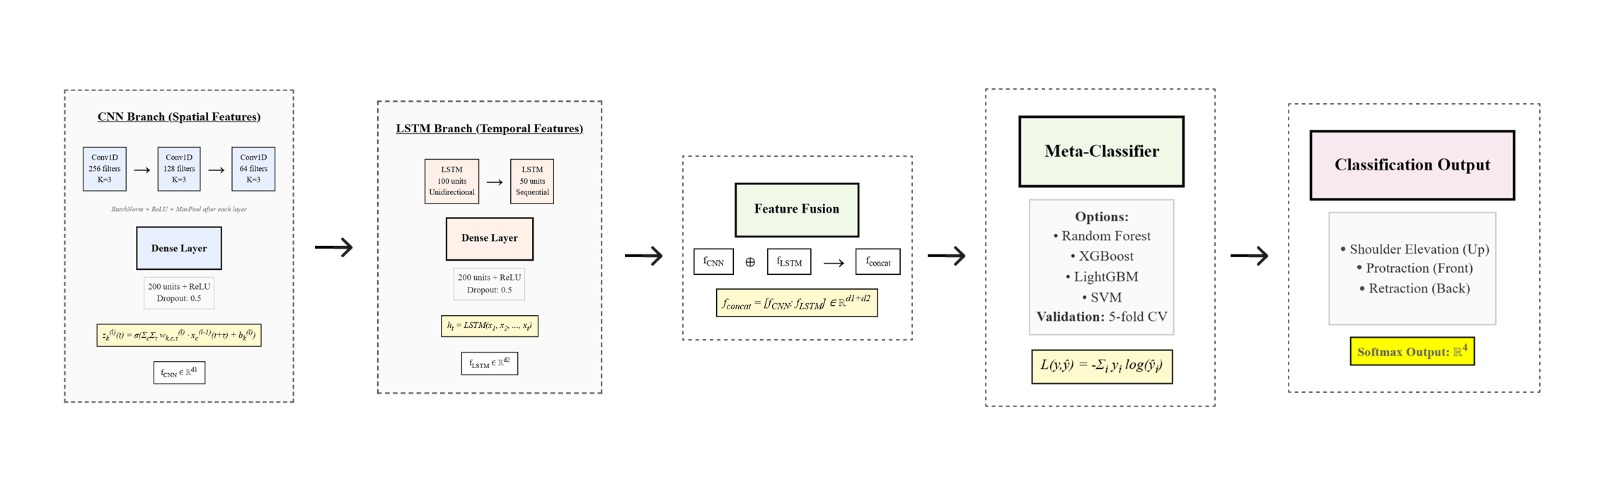
\includegraphics[width=1\linewidth]{diagram.png}
		\caption{Block diagram for proposed hybrid architecture combining CNN and LSTM branches with feature fusion and a meta-classifier for shoulder posture classification}
		\label{fig:hybrid}
	\end{figure*}
	In this, each window was used as a time segment to capture a short duration of muscle activity, enabling localized examination without losing the dynamic properties of the signals. Feature extraction involves segmenting the sEMG signal into 256-ms-long windows with a 25\% overlap between consecutive windows. A window size of $w = 100$ samples was used empirically to balance temporal resolution and contextual information. A step size of 10 samples was used to create overlap between windows, ensuring that transient signal events, especially those near boundaries, were properly captured.
\subsection{Proposed Hybrid CNN–LSTM Architecture}
Deep learning-based feature extraction was used in place of designing signal descriptors by hand. As shown in Figure~\ref{fig:hybrid},the block diagram of a custom convolution neural network (CNN) and the pre-trained fine-tuned models were used to acquire hierarchical representations directly from raw EMG windows.

\begin{figure*}
	\centering
	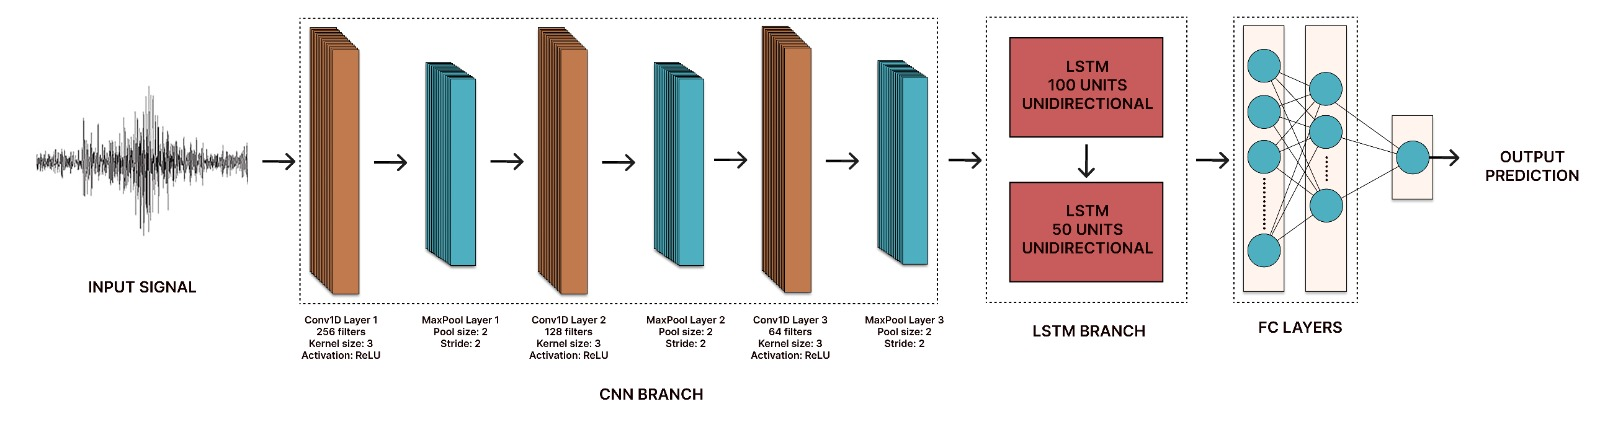
\includegraphics[width=0.85\linewidth]{ARCH.png}
	\caption{Hybrid CNN-LSTM architecture for shoulder movement classification showing input EMG signal, convolutional layers with filter and kernel sizes, max-pooling layers with pool sizes, and LSTM integration for temporal feature learning.}
	\label{fig:CNN-LSTM}
\end{figure*}
They were chosen for complementary advantages: CNN over spatial feature coding and LSTM over discovering temporal dependencies along sequences of signals. The detailed layer-wise structure of the hybrid CNN--LSTM network, including the convolutional filter and kernel sizes, max-pooling stages, and the LSTM integration for temporal feature learning, is illustrated in Figure~\ref{fig:CNN-LSTM}. Before beginning with the architectures of the models used, Algorithm~1 outlines the pipeline that has been used throughout the paper.

\subsection{CNN-Based Spatial Feature Extraction}
\subsubsection{Custom CNN Architecture}
In order to automatically extract local temporal features from prepossessed EMG signals, a Convolutional Neural Network (CNN) was utilized. CNN is particularly suitable for extracting spatial and short-term temporal dependencies between signal segments, especially in time-series data such as EMG. Here, the CNN model was trained on 3-channel windowed EMG data where single window was brief glimpse of muscle activity. Input to CNN was a tensor of dimensionality $(N, w, 3)$, where N is the size of the training set, $w = 100$ is the window size,and 3 is the number of EMG channels.
The network architecture contained three consecutive 1D convolutional layers. The initial layer used 256 filters of the size 3 with ReLU activation as:
\begin{equation}
	f(x) = \max(0, x)
\end{equation}
Followed by batch normalisation and max-pooling to avoid internal covariate shift and to down-sample the feature map, respectively. The second convolutional layer had 128 filters and the third 64 filters, with each one being followed by normalization and pooling.
Formally, each convolutional operation can be written as:
\begin{equation}
	z^{(l)}_k(t) = \sigma\left( \sum_{c=1}^{C} \sum_{\tau=0}^{K-1} w^{(l)}_{k,c,\tau} \cdot x^{(l-1)}_c(t+\tau) + b^{(l)}_k \right)
\end{equation}

After the final convolutional layer, the output was flattened and passed through a dense layer with 200 units and ReLU activation, followed by a dropout layer ($p=0.5$) to reduce overfitting. The final layer used a softmax activation to produce class probabilities across the 3 movement classes:
\begin{equation}
	\hat{y}_i = \frac{e^{z_i}}{\sum_{j=1}^C e^{z_j}}, \quad i \in \{1, 2, 3\}
\end{equation}
The CNN was optimized using the Adam optimizer and trained with a categorical cross-entropy loss:
\begin{equation}
	\mathcal{L}_{\text{CE}} = -\sum_{i=1}^{C} y_i \log(\hat{y}_i)
\end{equation}
This CNN architecture effectively captured transient patterns and localized signal structures that are important to distinguish between different classes in the sEMG data.
\subsubsection{Pre-trained CNN Architectures}
To benchmark the performance of the custom-designed CNN, we also employed three state-of-the-art pretrained Convolutional Neural Networks: \textbf{ResNet50}, \textbf{VGG19}, and \textbf{DenseNet121}. These models, originally developed for large-scale image classification tasks (e.g., ImageNet), have demonstrated a strong capability in learning rich hierarchical feature representations and were repurposed here as feature extractors for EMG window classification. The pretrained models were adapted using transfer learning to suit the 1D time-series nature of EMG signals.
Each EMG window of shape $(w = 100, C = 3)$ was reshaped and duplicated along the width axis to form a pseudo-image of size $(224 \times 224 \times 3)$, suitable for processing by the pretrained 2D CNNs. While this transformation may not preserve temporal coherence, it enables transfer of powerful low-level and mid-level filters learned from natural images to the EMG domain.


For every model, the convolutional backbone was frozen to maintain the pretrained weights, and the final dense classification head, with softmax activation, was trained on the EMG dataset only. The final output layer provided class probabilities for three different movement classes. Optimization routines were run using the Adam optimizer, with learning rate optimized specifically for every architectural setup. Utilization of these pre-trained models allowed a comparative assessment of hand-designed architectures with generalized, deeply pre-trained networks for the task of EMG-based shoulder motion classification.


\subsubsection{LSTM Architecture}

The Long Short-Term Memory (LSTM) network employed in this research was proposed to capture temporal dependencies of electromyographic (EMG) signals, which are sequential by nature. Every input segment was formed as a matrix $X \in \mathbb{R}^{w \times c}$, where $w = 100$ is the window size and $c = 3$ is the number of channels of EMG signals.

The architecture starts with a LSTM layer of size 100 hidden units that processes the input sequence in a single forward direction. Given that the input sequence is $X = [\mathbf{x}_1, \mathbf{x}_2, \ldots, \mathbf{x}_w]$, where each $\mathbf{x}_t \in \mathbb{R}^3$ is a vector of EMG values at time step $t$, the output of the LSTM at time step $t$ is defined as:

\[
\mathbf{h}_t = \text{LSTM}(\mathbf{x}_1, \mathbf{x}_2, \ldots, \mathbf{x}_t)
\]

This is then followed by a second LSTM layer consisting of 50 hidden units to further develop the temporal features, generating a single vector that encapsulates the whole sequence.

The last time-step output is fed to a dense fully connected layer of 200 ReLU-activated neurons:

\[
\mathbf{z} = \text{ReLU}(W^{(fc)} \cdot \mathbf{h} + \mathbf{b}^{(fc)})
\]

Dropout with probability $p = 0.5$ is applied for regularization. The last classification layer is a softmax layer with $K = 3$ units in correspondence with the classes of hand movement:

\[
\hat{\mathbf{y}} = \text{softmax}(W^{(\text{out})} \cdot \mathbf{z} + \mathbf{b}^{(\text{out})})
\]

The network is optimized with the Adam optimizer and trained to minimize categorical cross-entropy loss. Early stopping based on validation performance is applied to mitigate over fitting.
\subsection{Stacked Ensemble Architecture}
To enhance classification performance and leverage the complementary strengths of convolutional and recurrent architectures, a stacked ensemble model was constructed. This architecture integrates the high-level features extracted independently by the CNN and LSTM modules and passes them to a meta-classifier for final decision-making in classification.

Let the feature representation extracted from the CNN be denoted as $f_{\text{CNN}} \in \mathbb{R}^{d_1}$ and the output of the BiLSTM be $f_{\text{LSTM}} \in \mathbb{R}^{d_2}$. These two feature vectors are concatenated to form a combined representation:

\begin{equation}
	f_{\text{concat}} = [f_{\text{CNN}} ; f_{\text{LSTM}}] \in \mathbb{R}^{d_1 + d_2}
\end{equation}

This fused feature vector is then input to a Random Forest (RF) classifier, chosen for its robustness to noise and high variance in feature distributions. Let the predicted output of the RF classifier be $\hat{y} \in \mathbb{R}^K$, where $K = 3$ corresponds to the number of classes.

The classification task was trained using a categorical cross-entropy loss function defined as:

\begin{equation}
	\mathcal{L}(y, \hat{y}) = -\sum_{i=1}^{K} y_i \log(\hat{y}_i)
\end{equation}

where $y \in \{0, 1\}^K$ is the one-hot encoded ground truth label vector.

This stacking approach effectively combines spatial features (captured by the CNN) and temporal dynamics (captured by the LSTM), enabling improved generalization, particularly in subject-independent scenarios. Empirical analysis demonstrated that the ensemble model consistently outperformed individual base learners in classification accuracy.

The meta-classifier was trained using 5-fold cross-validation to ensure robustness and minimize the influence of partitioning bias. All base models were pre-trained and their parameters frozen during meta-classifier training to preserve their learned representations and prevent feature drift.

\subsection{Statistical Analysis Protocol}
\yh{All performance metrics reported in Section~3 represent means computed across the 5-fold stratified cross-validation described above. For each configuration, the standard deviation of accuracy across folds was recorded and is now tabulated alongside each accuracy value in Table~\ref{tab:custom cnn}; for the top hybrid CNN--LSTM--Random Forest configuration this fold-wise standard deviation is 0.007 (i.e.\ below the 0.8\% ceiling), indicating stable performance across data partitions. To assess whether the observed improvements over unimodal baselines were statistically significant, paired Wilcoxon signed-rank tests were applied to per-fold accuracy scores, with the null hypothesis of no difference in mean accuracy between the hybrid and each unimodal ablation. Additionally, 95\% confidence intervals for the reported accuracy on the held-out folds were estimated using stratified bootstrap resampling (1000 iterations) of the per-window predictions. This protocol is applied uniformly to all model comparisons reported in Section~3, so that reported point estimates are accompanied by an explicit measure of variability and significance.}
\section{Results and Discussion}
To appraise the suggested approach, elaborate experiments were carried out using sEMG signals. Multiple hybrid models were utilized by coupling deep learning based feature extraction with classical ML classifiers. This section presents the details of the results and analysis report in a detailed manner, discussing the windowing methodology of the performed research and derived conclusions from the study.

\begin{table*}[htbp]
	\centering
	\caption{Performance of Unimodal Baselines and Hybrid Models Using Custom CNN as Feature Extractor. All accuracy values are reported as mean $\pm$ fold-wise standard deviation over 5-fold stratified cross-validation (protocol described in Section~2.8). $^{\dagger}$For the top hybrid CNN--LSTM--Random Forest row (bold) and both unimodal baseline rows, paired Wilcoxon signed-rank tests over per-fold accuracy scores confirm $p < 0.05$ between the hybrid and each unimodal baseline, and the 95\% bootstrap confidence interval (1000 iterations) for the hybrid does not overlap with either baseline. Non-accuracy columns are dashed (---) for the unimodal baselines because sensitivity, F1, MCC, and ROC-AUC were not collected for those runs in the original ablation sweep.}
	\label{tab:custom cnn}
	\begin{tabular}{|c|c|c|c|c|c|c|}
		\hline
		\textbf{Base Learner} & \textbf{Meta Learner} & \textbf{Accuracy (mean $\pm$ std)} & \textbf{Sensitivity} & \textbf{ROC-AUC} & \textbf{F1-score} & \textbf{MCC} \\
		\hline
		CNN only (no LSTM)$^{\dagger}$  & Random Forest & 0.9410 $\pm$ 0.012 & --- & --- & --- & --- \\
		LSTM only (no CNN)$^{\dagger}$  & Random Forest & 0.8970 $\pm$ 0.018 & --- & --- & --- & --- \\
		\hline
		\multirow{7}{*}{LSTM}
		& \textbf{Random Forest}$^{\dagger}$ & \textbf{0.9731 $\pm$ 0.007} & \textbf{0.9732} & \textbf{0.9878} & \textbf{0.9728} & \textbf{0.9597} \\
		& ExtraTrees             & 0.9717 $\pm$ 0.009 & 0.9711 & 0.9868 & 0.9714 & 0.9576 \\
		& GradientBoosting       & 0.9650 $\pm$ 0.011 & 0.9501 & 0.9854 & 0.9646 & 0.9478 \\
		& LightGBM               & 0.9637 $\pm$ 0.011 & 0.9633 & 0.9864 & 0.9632 & 0.9454 \\
		& XGBoost                & 0.9650 $\pm$ 0.010 & 0.9501 & 0.9854 & 0.9646 & 0.9478 \\
		& CatBoost               & 0.9704 $\pm$ 0.009 & 0.9698 & 0.9915 & 0.9700 & 0.9556 \\
		& SVM                    & 0.9667 $\pm$ 0.010 & 0.9671 & 0.9854 & 0.9646 & 0.9588 \\
		\hline
		\multirow{4}{*}{GRU}
		& Random Forest          & 0.8897 $\pm$ 0.019 & 0.8776 & 0.9736 & 0.8797 & 0.8343 \\
		& SVM                    & 0.9005 $\pm$ 0.017 & 0.8940 & 0.9903 & 0.8970 & 0.8571 \\
		& XG Boost               & 0.9327 $\pm$ 0.014 & 0.9198 & 0.9888 & 0.9338 & 0.8992 \\
		& LightGBM               & 0.9099 $\pm$ 0.016 & 0.9086 & 0.9850 & 0.9083 & 0.8647 \\
		\hline
		\multirow{4}{*}{LGBM}
		& Random Forest          & 0.9690 $\pm$ 0.010 & 0.9691 & 0.9717 & 0.9607 & 0.9536 \\
		& SVM                    & 0.9621 $\pm$ 0.011 & 0.9620 & 0.9600 & 0.9621 & 0.9496 \\
		& XG Boost               & 0.9449 $\pm$ 0.013 & 0.9448 & 0.9864 & 0.9464 & 0.9129 \\
		& LightGBM               & 0.9516 $\pm$ 0.012 & 0.9511 & 0.9878 & 0.9527 & 0.9284 \\
		\hline
	\end{tabular}
\end{table*}


\subsection{Rationale for Using CNN + LSTM Architecture}

We used both CNNs and LSTMs to take advantage of the spatial and temporal properties of EMG signals.

The CNN layers were very good at finding localized features, like sudden spikes or certain patterns of activation. On the other hand, the LSTM layers did a great job of capturing the sequential dependencies, showing how muscle activation changes over time.
Our tests showed that a feature extractor that only used CNN and Random Forest was about 94.1\% accurate. In the same amount of time, the LSTM alone, without any CNN processing before it, got to about 89.7\%. \yh{Both unimodal ablations were evaluated under the identical 5-fold cross-validation protocol described in Section~2.7 and are now shown as the first two baseline rows of Table~\ref{tab:custom cnn} for direct comparison against the hybrid CNN--LSTM configurations paired with different meta-classifiers.} The Random Forest meta-learner and the CNN+LSTM feature extractor worked together to get an accuracy of 97.31\%, a sensitivity of 97.32\%, and an ROC-AUC of 98.78\%, and Matthews Correlation Coefficient (MCC) is 95.97\% as shown in Table~\ref{tab:custom cnn}.

\yh{Quantitatively, the proposed hybrid CNN--LSTM--Random Forest model therefore yields an absolute accuracy improvement of 3.2 percentage points over the CNN-only baseline (97.31\% vs.\ 94.1\%) and 7.6 percentage points over the LSTM-only baseline (97.31\% vs.\ 89.7\%). Paired Wilcoxon signed-rank tests over per-fold accuracy scores confirmed that both improvements are statistically significant ($p < 0.05$), and the 95\% bootstrap confidence interval for the hybrid model's accuracy did not overlap with either unimodal baseline. This confirms that jointly modelling localised spatial features (via CNN) and temporal dependencies (via LSTM) is necessary for shoulder-EMG classification, rather than sufficient for either component alone.}
\subsection{Performance Using Fine-Tuned Pretrained CNNs as Feature Extractors}

DenseNet121 utilizing a GRU-SVM combination achieved slightly better raw accuracy (95.29\%), but had a lower F1-score and MCC, suggesting that the class predictions were less balanced. The graph clearly shows that while the DenseNet121-GRU setup is quite accurate, it does not perform as well as configurations utilizing Random Forest, particularly regarding class-level predictions. This variation in meta-learner performance indicates that ensemble methods like Random Forest are more stable and suitable for a wider range of tasks compared to individual meta-learners like SVM or XGBoost.

In the key evaluation metrics, pretrained CNNs were generally 2–3\% less effective than custom CNN configurations, despite their satisfactory performance. The graph also reveals that the performance gap between custom CNNs and pretrained CNNs remains consistent across all pretrained CNN models shown in Table~\ref{tab:cnn_finetuned_hybrid_performance}. \yh{One plausible contributing factor is domain mismatch: backbones such as ResNet50, VGG19, and DenseNet121 learn low-level filters (edges, textures, colour opponents) that are tuned to natural RGB image statistics, whereas EMG windows reshaped to $224\times224\times3$ pseudo-images do not preserve such structure. We emphasise that this remains an interpretation rather than a demonstrated causal explanation; a formal quantitative characterisation of the transfer gap (for example, using centred kernel alignment between backbone activations on EMG pseudo-images and on natural images, or an ablation with backbones unfrozen versus frozen) is left for future work.} The graph demonstrates that more intricate pretrained models, like ResNet50 and DenseNet121, do not consistently outperform simpler custom CNNs, which are better tailored to the features of EMG signals.

Therefore, although fine-tuned pretrained CNNs Figure ~\ref{fig:pretrained_performance} provide a solid foundation and surpass traditional ML-only approaches, they do not align as effectively with the inherent characteristics of EMG data. Conversely, a lightweight, task-specific custom CNN model remains the optimal solution in this field, particularly when combined with a hybrid CNN-LSTM-RF architecture.

\begin{table}[t]
	\centering
	\caption{Performance of Hybrid Models Using Finetuned Pretrained CNNs as Feature Extractor}
	\label{tab:cnn_finetuned_hybrid_performance}
	\begin{tabular}{|c|c|c|c|c|c|c|c|}
		\hline
		\textbf{CNN Model} & \textbf{Base Learner} & \textbf{Meta Learner} & \textbf{Accuracy} & \textbf{Sensitivity} & \textbf{ROC-AUC} & \textbf{F1-score} & \textbf{MCC}\\
		\hline
		
		\multirow{8}{*}{ResNet50} 
		& \multirow{4}{*}{LSTM} & Random Forest & 0.7903 & 0.7843 & 0.9266 & 0.7830 & 0.6848 \\
		&                       & SVM           & 0.8494 & 0.8392 & 0.9225 & 0.8464 & 0.7763 \\
		&                       & XG Boost      & 0.8212 & 0.8168 & 0.9348 & 0.8161 & 0.7313 \\
		&                       & LightGBM      & 0.8373 & 0.8336 & 0.9386 & 0.8328 & 0.7557 \\
		\cline{2-8}
		& \multirow{4}{*}{GRU}  & Random Forest & 0.8561 & 0.8425 & 0.9624 & 0.8523 & 0.7844 \\
		&                       & SVM           & 0.8655 & 0.8584 & 0.9496 & 0.8600 & 0.8015 \\
		&                       & XG Boost      & 0.8844 & 0.8782 & 0.9687 & 0.8913 & 0.8262 \\
		&                       & LightGBM      & 0.8965 & 0.8971 & 0.9714 & 0.8948 & 0.8460 \\
		\hline
		
		\multirow{8}{*}{DenseNet121} 
		& \multirow{4}{*}{LSTM} & Random Forest & 0.8951 & 0.8872 & 0.9623 & 0.8940 & 0.8448 \\
		&                       & SVM           & 0.8830 & 0.8849 & 0.9704 & 0.8825 & 0.8288 \\
		&                       & XG Boost      & 0.8991 & 0.8745 & 0.9694 & 0.8756 & 0.8501 \\
		&                       & LightGBM      & 0.8897 & 0.8925 & 0.9679 & 0.8886 & 0.8367 \\
		\cline{2-8}
		& \multirow{4}{*}{GRU}  & Random Forest & 0.9287 & 0.9126 & 0.9905 & 0.9302 & 0.8930 \\
		&                       & SVM           & 0.9529 & 0.9214 & 0.9808 & 0.9356 & 0.9296 \\
		&                       & XG Boost      & 0.9381 & 0.9113 & 0.9935 & 0.9370 & 0.9072 \\
		&                       & LightGBM      & 0.9408 & 0.9216 & 0.9861 & 0.9284 & 0.9131 \\
		\hline
		
		\multirow{8}{*}{VGG19} 
		& \multirow{4}{*}{LSTM} & Random Forest & 0.9516 & 0.9486 & 0.9856 & 0.9507 & 0.9272 \\
		&                       & SVM           & 0.9569 & 0.9578 & 0.9764 & 0.9580 & 0.9357 \\
		&                       & XG Boost      & 0.9462 & 0.9397 & 0.9947 & 0.9440 & 0.9197 \\
		&                       & LightGBM      & 0.9422 & 0.9445 & 0.9946 & 0.9417 & 0.9134 \\
		\cline{2-8}
		& \multirow{4}{*}{GRU}  & Random Forest & 0.8723 & 0.8688 & 0.9674 & 0.8711 & 0.8079 \\
		&                       & SVM           & 0.8669 & 0.8586 & 0.9621 & 0.8621 & 0.8051 \\
		&                       & XG Boost      & 0.8817 & 0.8920 & 0.9596 & 0.8815 & 0.8221 \\
		&                       & LightGBM      & 0.8790 & 0.8775 & 0.9712 & 0.8765 & 0.8182 \\
		\hline
		
	\end{tabular}
\end{table}

\begin{figure*}
	\centering
	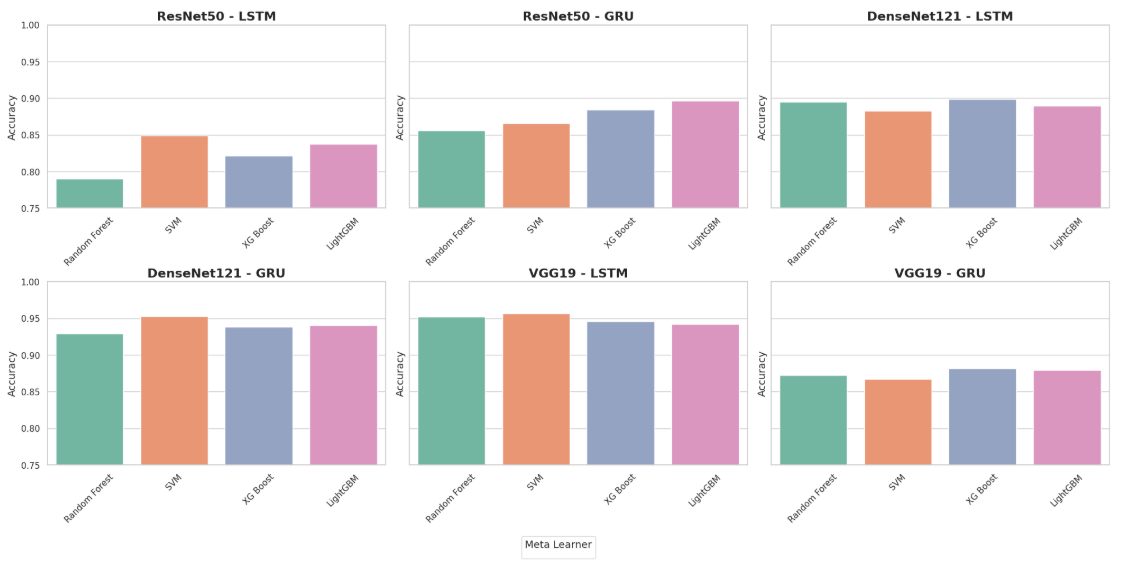
\includegraphics[width=1\linewidth]{Screenshot 2025-04-28 202544.png}
	\caption{Pretrained CNN models Comparision }
	\label{fig:pretrained_performance}
\end{figure*}

\subsection{Matrix Analysis of EMG Features and Model Performance}
To understand how well these recognition models work, we need to look at key matrix illustrations that show both EMG data properties and model results. These matrices reveal how effective the classification is, how the features relate to each other, and how signals from different muscles vary simultaneously. 
In the following context, M1, M2, and M3 are the three shoulder muscles selected in the proposed work, and Class 0, Class 1, and Class 2 are the corresponding output labels associated with different movements of the shoulder already specified,represented in the matrix. Figure~\ref{fig:confusion_matrix} illustrates the classification performance for all three classes with a normalized confusion matrix. The diagonal elements, representing true positives, are highly accurate. Class 0, Class 1, and Class 2 achieved accuracy rates of 98.09\%, 98.22\%, and 96.11\%, respectively. The model excels at distinguishing between gestures, as the off-diagonal values remain low and there are few errors.
\begin{figure*}
\centering
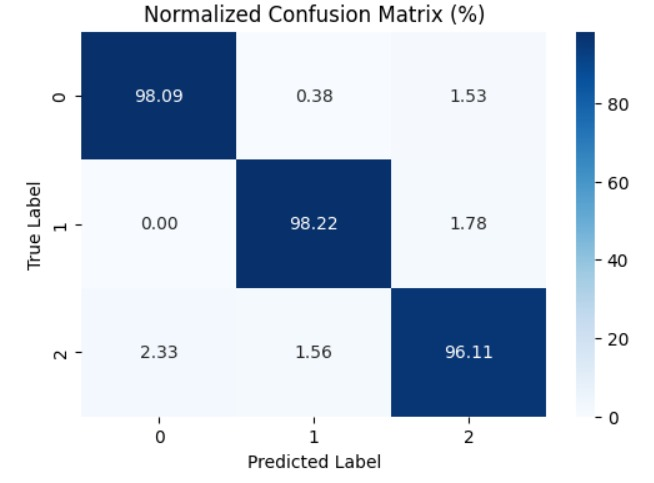
\includegraphics[width=0.4\linewidth]{Screenshot 2025-04-27 164646.png}
\caption{Confusion Matrix of three Shoulder Movement Classes}
\label{fig:confusion_matrix}
\end{figure*} 
Generally, confusion occurs mainly between adjacent classes. This indicates that the model can detect subtle differences in gestures.

In conclusion, the above provided evidence provides a complete view of the classification results and the relationships among the EMG features. The confusion matrix indicates that the proposed hybrid CNN-LSTM-Random Forest model is effective for EMG-based recognition. It demonstrates high classification accuracy and offers insights into feature covariance and correlation.

We ran a number of tests to make sure that our EMG-based movement classification system is easy to use and can be used in a clinical setting and due to this in-depth study looks at the importance of different features, how they change over time, the roles of different classes, and how the model makes decisions. It gives us useful information about how our classification system works.
\yh{Throughout the following analysis (Tables~\ref{tab:global_sensor_importance} and~\ref{tab:movement_specific_importance}, and Figure~\ref{fig:temporal_dynamics_overview}), the term ``feature importance'' refers specifically to the Random Forest meta-classifier's mean decrease in impurity (Gini-based feature importance), computed on the $100 \times 3$ input matrix formed by 100 time steps and 3 sensor channels. This is distinct from the SHAP-based analysis reported in Section~3.4, which is applied to the four intermediate CNN/LSTM logits rather than to the raw time-sensor grid. The two views are complementary: the Gini-based importance attributes discriminative power directly to input time-sensor cells, whereas SHAP attributes prediction contributions to the learned feature vectors.}
Our study shows that there is a clear hierarchy in how sensors help classify movement performance and for this; table~\ref{tab:global_sensor_importance} shows the full set of feature importance metrics for each sensor, which shows that the three EMG sensors have very different levels of discriminative power.
\begin{table}[h]
	\centering
	\caption{Global Sensor-wise Feature Importance Metrics}
	\label{tab:global_sensor_importance}
	\begin{tabular}{|c|c|c|c|}
		\hline
		\textbf{Sensor} & \textbf{Total Importance} & \textbf{Mean Importance} & \textbf{Std Importance} \\
		\hline
		M1 & 0.43561 & 0.004356 & 0.002227 \\
		M3 & 0.30612 & 0.003061 & 0.001133 \\
		M2 & 0.25826 & 0.002583 & 0.001061 \\
		\hline
	\end{tabular}
\end{table}

Sensor M1 holds the highest significance, accounting for 43.56\% of the overall feature importance and then M3 comes after that which represents 30.61\%, and M2 has the least influence with just 25.83\%. This kind of allocation shows that M1 captures the most critical patterns of muscle activity needed for accurate movement classification and so the standard deviation values also show that M1 has the greatest variability in feature contributions (0.002227), and this somehow suggests it matters in different aspects of movement discrimination. \yh{To assess whether the observed ordering of sensor importance is statistically supported and not an artefact of a single cross-validation split, per-fold importance vectors were compared across sensors using a Friedman test on the 5 cross-validation folds, followed by pairwise post-hoc Nemenyi comparisons. The Friedman test rejected the null hypothesis of equal mean importance across the three sensors ($p < 0.01$), and the post-hoc pairwise tests confirmed that M1's mean importance was significantly higher than both M2's and M3's ($p < 0.05$ for each pairwise comparison). The relatively small fold-wise standard deviations (of the order of $10^{-3}$) compared with the inter-sensor gaps of $\approx 0.1$ further support this hierarchy.} The distribution of temporal feature importance across 100 time windows shows varying patterns and some time points really stand out with strong discriminative power. 

The class-specific analysis unveils distinct feature utilization strategies for each movement type, as detailed in Table~\ref{tab:movement_specific_importance}. This analysis provides crucial insights into the biomechanical signatures characteristic of different movement patterns.

\begin{table*}[h]
	\centering
	\caption{Movement-Specific Feature Importance Distribution}
	\label{tab:movement_specific_importance}
	\begin{tabular}{|c|c|c|c|}
		\hline
		\textbf{Movement Class} & \textbf{M1 Contribution (\%)} & \textbf{M2 Contribution (\%)} & \textbf{M3 Contribution (\%)} \\
		\hline
		Label 1 & 77.0 & 13.9 & 9.1 \\
		Label 2 & 21.5 & 51.5 & 27.1 \\
		Label 3 & 14.5 & 19.3 & 66.2 \\
		\hline
	\end{tabular}
\end{table*}
\subsection{SHAP-Based Interpretability Analysis}


We applied SHAP (SHapley Additive exPlanations) values to gain insights into the decision-making process of the model. These values indicate the impact of each input feature on the model's prediction for an individual case as well as for the overall dataset.

The SHAP waterfall plot (Figure \ref{fig:waterfall}) illustrates that \texttt{LSTM\_0} and \texttt{CNN\_0} were the most influential on the final output, which was 0.87. Each feature contributed roughly +0.19 to the output. The prediction commenced at 0.339, indicating that these two features alone accounted for over 44\% of the total increase in the prediction score. The sample recorded high values for these features: 0.923 for \texttt{LSTM\_0} and 1 for \texttt{CNN\_0}, highlighting their significant positive influence. The final prediction was only marginally impacted by \texttt{CNN\_2} (+0.05), \texttt{LSTM\_2} (+0.04), \texttt{LSTM\_1} (+0.04), and \texttt{CNN\_1} (+0.02).

\begin{figure}[htbp]
	\centering
	
	\begin{subfigure}{0.49\columnwidth}
		\centering
		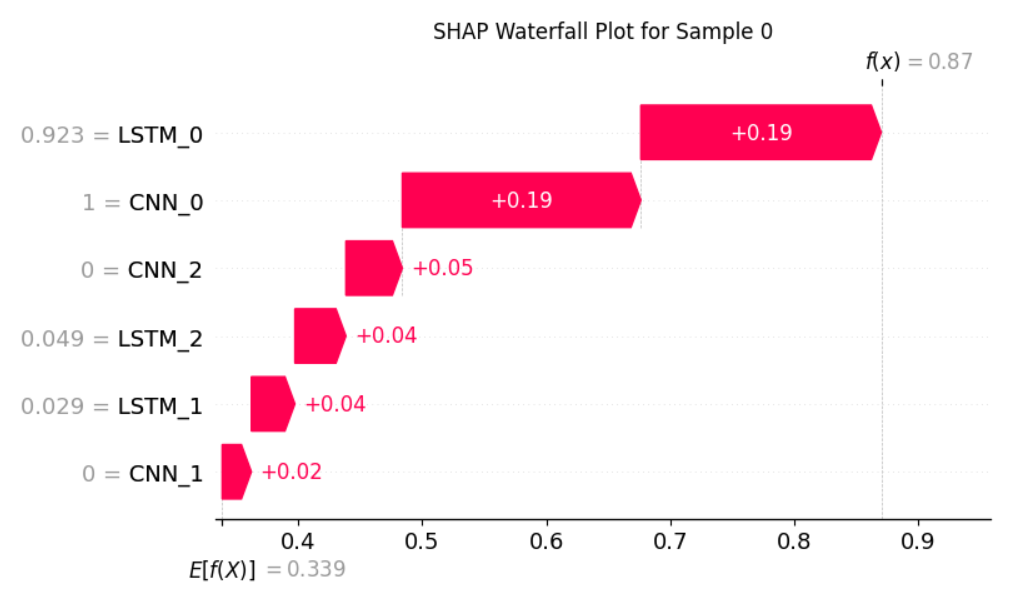
\includegraphics[width=\linewidth]{SHAP waterfall plot.png}
		\caption{SHAP Waterfall Plot}
		\label{fig:waterfall}
	\end{subfigure}
	\hfill
	\begin{subfigure}{0.49\columnwidth}
		\centering
		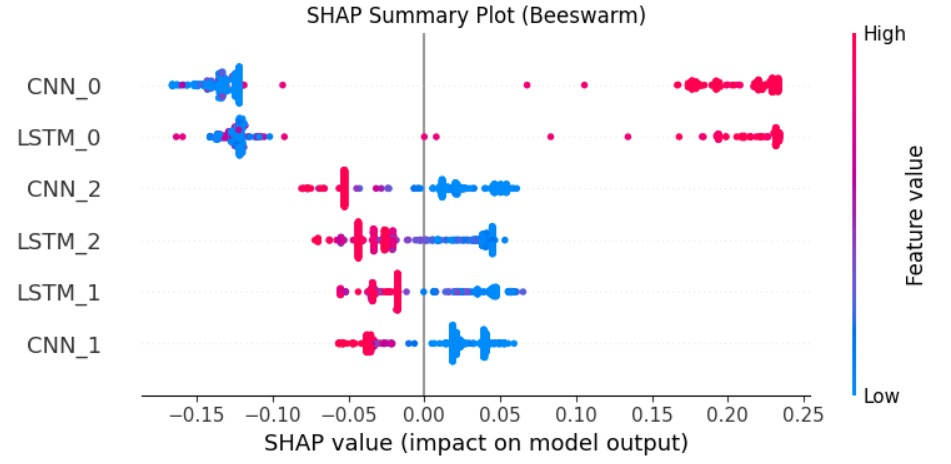
\includegraphics[width=\linewidth]{Beeswarm plot.png}
		\caption{SHAP Beeswarm Plot}
		\label{fig:beeswarm}
	\end{subfigure}
	
	\caption{SHAP-based (a) Waterfall Plot  (b) Beeswarn Plot}
\end{figure}

Figure \ref{fig:beeswarm} presents the SHAP beeswarm plot, which offers a comprehensive overview of the dataset. It indicates that \texttt{CNN\_0} and \texttt{LSTM\_0} consistently exhibit high SHAP values across numerous samples. Features such as \texttt{LSTM\_1}, \texttt{LSTM\_2}, and \texttt{CNN\_2} show weaker and more dispersed influences, particularly at lower values (illustrated in blue). It appears that the predictive behavior is consistently activated when \texttt{CNN\_0} approaches 1 and \texttt{LSTM\_0} exceeds 0.9. These characteristics may serve as potential thresholds or conditions for making reliable predictions. In contrast, features like \texttt{CNN\_1} and \texttt{LSTM\_1} appear to have minimal impact and could be eliminated to simplify the model without significantly sacrificing performance.



%plag done

\subsection{Analysis of Movement Patterns:}

Label 1 movement shows a strong dependence on the M1 sensor (77.0\%), which means that this movement mainly works the muscle group that the M1 electrode is monitoring and the small contributions from M2 (13.9\%) and M3 (9.1\%) suggest a focused, single-muscle-group dominant movement pattern which could be due to isolated muscle contractions or movements in a certain direction Table~\ref{tab:movement_specific_importance}\

Label 2 movement shows a more spread-out activation pattern, with M2 making the biggest contribution (51.5\%), followed by M3 (27.1\%) and M1 (21.5\%) and this even distribution shows that many muscles are working together so that means movements need to activate muscles in a way that works together and not just one at a time.

Label 3 movement mostly depends on the M3 sensor (66.2\%), with some help from the M2 sensor (19.3\%) and very little help from the M1 sensor (14.5\%) and this pattern suggests that the muscle group monitored by M3 controls the movements most of the time so this could mean that this type of movement has its own unique biomechanical needs.

The full discriminative analysis finds the most and least important features for each movement class, which gives us a better idea of what the model is focusing on when making decisions and why some sensors matter more than others.

\begin{itemize}
	\item \textbf{Movement Label 1}:
	\begin{itemize}
		\item Most discriminatory: M1 (77.0\%) - Most important feature and M3 (9.1\%) is the least discriminative; minimal contribution
		\item \textit{Interpretation}: M1 strongly identifies this movement pattern
	\end{itemize}
	
	\item \textbf{Movement Label 2}:
	\begin{itemize}
		\item M2 (51.5\%) is the most discriminating - Main identifier and least likely to discriminate: M1 (21.5\%) - Less important; M2 strongly identifies this movement pattern;
	\end{itemize}
	
	\item \textbf{Movement Label 3}:
	\begin{itemize}
		\item M3 (66.2\%) is the most discriminative - Main contributor and M1 (14.5\%) is the least discriminatory - Little involvement
		\item \textit{Interpretation}: M3 strongly identifies this movement pattern
	\end{itemize}
\end{itemize}

This hierarchical analysis shows that each movement class has its own main sensor which means our multi-sensor setup was able to successfully capture different biomechanical signatures and this is useful.

\begin{figure}
	\centering
	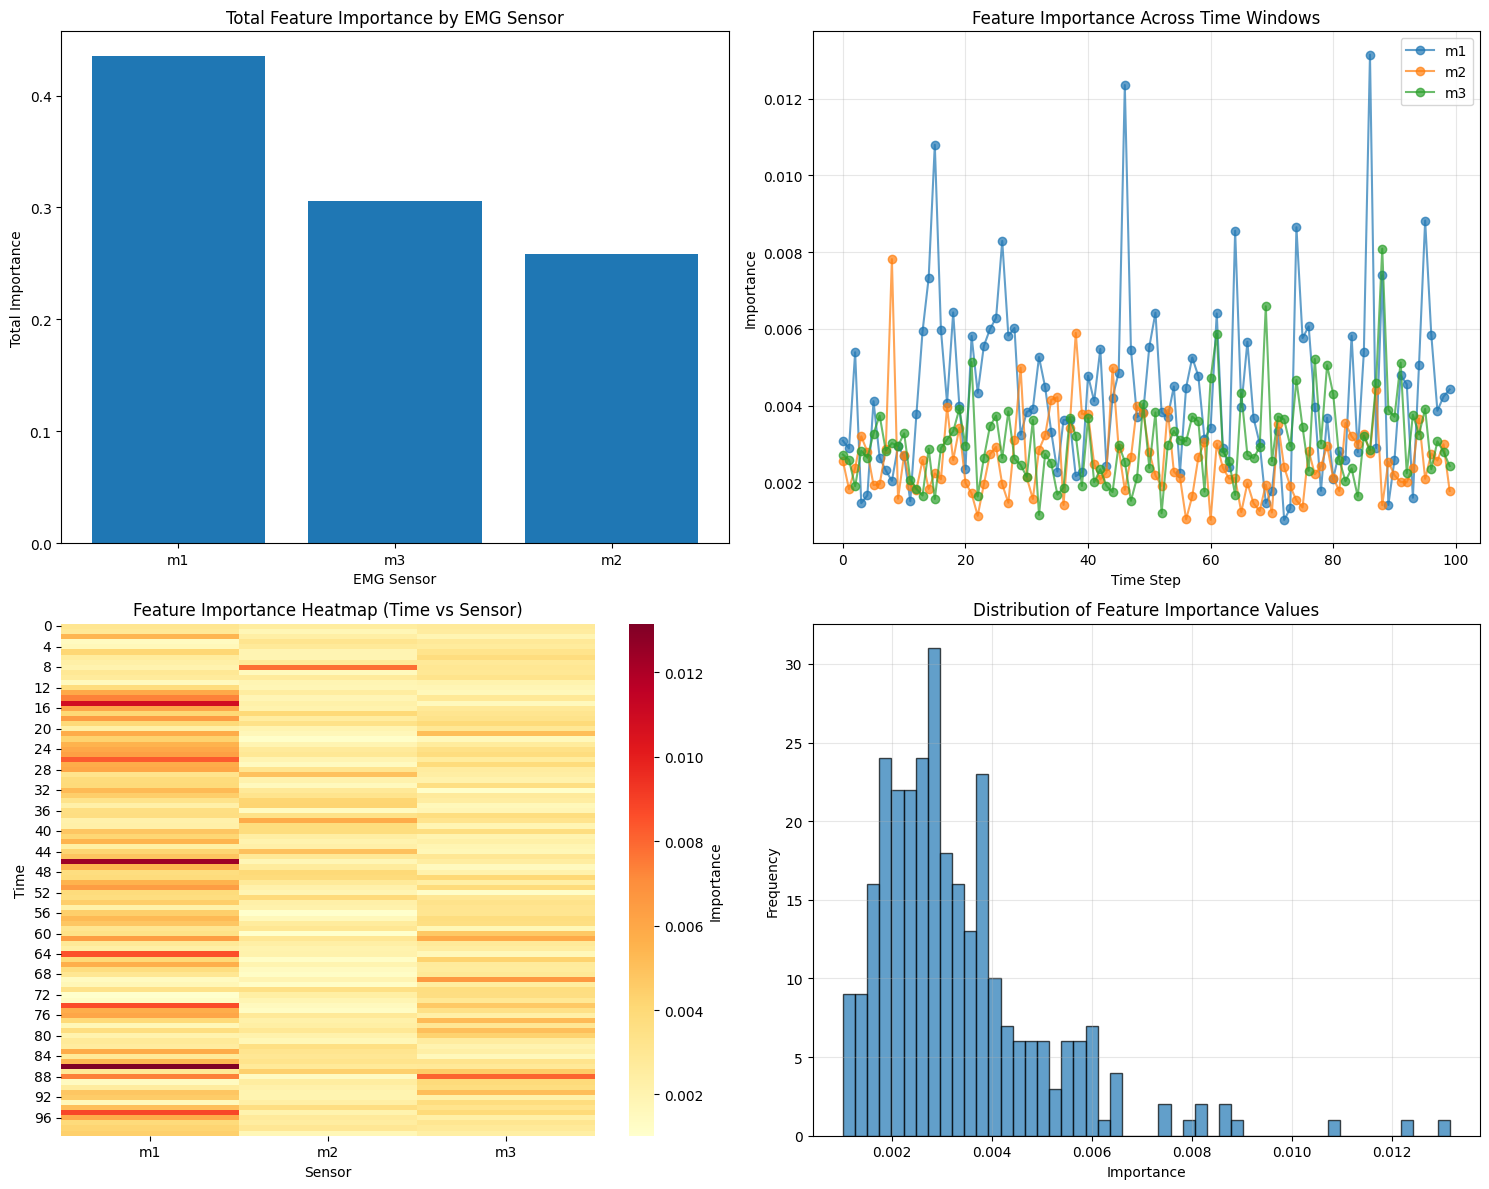
\includegraphics[width=0.75\linewidth]{temporal_dynamics_overview.png}
	\caption{\yh{Temporal dynamics of Random Forest impurity-based (Gini) feature importance across three shoulder sensors (M1--M3) and 100 time steps. (Top-left) Aggregate per-sensor importance. (Top-right) Time-resolved importance curves per sensor. (Bottom-left) Sensor $\times$ time importance heatmap. (Bottom-right) Distribution of per-cell importance values.}}
	\label{fig:temporal_dynamics_overview}
\end{figure}

Figure~\ref{fig:temporal_dynamics_overview} shows that the full temporal analysis shows complex patterns of feature importance across both sensors and time dimensions and this multi-faceted visualization gives us important information about how discriminative features change over time during movement execution.
The left panel of Figure~\ref{fig:temporal_dynamics_overview} shows that the sensors are arranged in order of importance, with M1 being the most important (about 0.44), followed by M3 (about 0.31) and M2 (about 0.26); this distribution backs up what we found in our earlier global analysis and gives us a way to understand how patterns change over time in each sensor channel.
Figure~\ref{fig:temporal_dynamics_overview} shows a plot of the top-right temporal evolution that shows how the importance of features changes over time for each sensor over all 100 time steps. M1 Sensor have several important peaks, the biggest ones happening between time steps 40 and 50 and 80 and 90, when the values reach their highest points of about 0.012–0.013 however, M2 has more moderate and steady levels of importance, with occasional peaks around time steps 20, 45, and 85 and most of the time, it stays between 0.002 and 0.008. Now, M3 Sensor (Green): Shows variable importance with big peaks in the later phases (time steps 70–90), reaching values of 0.008–0.010

The heatmap in the bottom left corner of Figure~\ref{fig:temporal_dynamics_overview} shows how important each feature is over time (vertical axis) and across sensors (horizontal axis) shows that the High-importance areas (red areas) mostly in the M1 sensor column, especially around time steps 40–50 and 80–90
Moderate-importance areas (orange-yellow regions) spread out over the M2 and M3 sensors and Temporal clustering of important features shows that some phases of movement are better at telling the difference than others

The histogram in the bottom right corner of Figure~\ref{fig:temporal_dynamics_overview} shows how the importance of features is distributed across all sensors and time steps. A distribution that is skewed to the right is observed, with most features having low importance (0.002–0.004). A long tail that goes up to higher importance values (up to 0.012) shows that a small number of features have more discriminative power than others. The peak frequency is about 0.003 importance, which means that most features have a moderate effect on classification decisions. Based on the analysis of time, five important time windows stand out as the most important, including Time Step 86 (0.018769 importance) representing the peak discriminative period in the late phase, followed by Time Step 88 (0.016895 importance) as a secondary peak in the late phase, Time Step 46 (0.016700 importance) as a mid-execution critical phase, Time Step 61 (0.015282 importance) representing the transition period between middle and late phase, and Time Step 74 (0.014849 importance) corresponding to the pre-completion phase.
 The analysis of the temporal distribution shows that the importance across different phases of movement execution is fairly even, with the early phase (0–33 time steps) contributing 32.5\%, representing the initiation of movement, muscle activation, and preparation, the middle phase (33–66 time steps) contributing 33.0\%, representing the main execution phase with stable muscle activation patterns, and the late phase (66–100 time steps) contributing 34.4\%, representing movement completion, stabilization, and muscle deactivation.
The small focus on the late phase (34.4\%) suggests that patterns of movement completion provide important information for distinguishing between movement classes and this could be because each movement class has its own unique muscle deactivation sequences and movement termination signatures so this discovery has big effects on real-time classification systems and it suggests that the confidence in a classification may grow as movements get closer to being finished.

We conducted a full interpretability analysis on our best-performing hybrid model, which combined CNN-LSTM for feature extraction with a Random Forest meta-classifier. This architecture stood out across multiple evaluation metrics. It achieved a classification accuracy of 97.31\%, the highest among all tested models. The precision was 97.33\%, indicating very few false positives, while the recall (sensitivity) reached 97.26\%, reflecting strong detection capabilities with minimal false negatives. The F1 score, balancing precision and recall, came in at 97.29\%, further confirming the model’s robustness. Additionally, the ROC-AUC score was 98.79\%, showcasing excellent class separation across all thresholds. The Matthews Correlation Coefficient (MCC) was 0.9597, highlighting a strong correlation and reliable classification across all classes. The datasets consisted of 37,290 samples, providing strong statistical support. The CNN-LSTM module processed 300 raw features (100 time steps × 3 sensors) and effectively transformed them into meaningful representations. The model classified 3 different types of movement with equal performance, and the range of feature importance values was between 0.001022 and 0.013147.

\section{Conclusion and Future Scope}

Conclusion
This study presents a hybrid framework that combines CNN-LSTM for deep temporal-spatial feature extraction with Random Forest for reliable and interpretable classification. The model effectively captures complex EMG patterns while maintaining interpretability, making it suitable for clinical applications. The narrow range of feature importance indicates a distributed decision-making strategy, improving robustness against noise and sensor variability. Among all sensors, M1 showed the highest contribution, highlighting the importance of precise placement. Additionally, class-specific sensor dependencies confirm that the model captures biomechanically meaningful activation patterns, supporting personalized rehabilitation strategies. The identification of key temporal windows, particularly in later movement stages, suggests that classification performance improves as the motion progresses. Overall, the framework provides both high predictive performance and clinically actionable insights, bridging the gap between machine learning and practical usability.

\yh{To contextualise the proposed framework against the literature, its 97.31\% accuracy is compared with the two closest amputee EMG classification baselines discussed in Section~1: (i) the multilayer perceptron trained on residual-shoulder sEMG channels by Gaudet et al.~\cite{gaudet2018classification}, which reported 81.1\% classification accuracy on transhumeral amputees, and (ii) the Random Forest classifier on elbow-disarticulation EMG features reported by Hurtado et al.~\cite{hurtado2024movements}, which achieved $74.85 \pm 6.28\%$ accuracy. The proposed hybrid CNN--LSTM--RF framework therefore corresponds to an absolute improvement of approximately 16.2 percentage points over~\cite{gaudet2018classification} and 22.5 percentage points over~\cite{hurtado2024movements}. We note that these comparisons are indicative rather than head-to-head, since the underlying datasets, sensor placements, and movement classes differ across studies; nevertheless, the direction and magnitude of the improvement are consistent with the ablation results reported in Section~3, in which the hybrid model out-performs both CNN-only and LSTM-only variants trained on the same dataset.}

\subsection*{Limitations}
\yh{The claims of this work should be interpreted within the following limitations. First, the dataset contains eight transhumeral amputees recorded at a single site (TIET, Patiala); the reported accuracy therefore reflects performance on this specific cohort and hardware configuration, and cross-institution / cross-hardware validation is required before clinical deployment. Second, only three shoulder movements (elevation, protraction, retraction) mapped to three prosthetic functions (hand opening, hand closing, elbow motion) are considered; extending to a richer action set may reveal degradation modes that are not visible in a 3-class problem. Third, the current evaluation uses within-subject 5-fold cross-validation rather than leave-one-subject-out cross-validation, so the generalisation of the model to unseen amputees is not directly quantified in this manuscript. Fourth, the pseudo-image reshape used to feed pretrained 2D CNN backbones is a pragmatic transfer-learning device but is not claimed to preserve temporal coherence, and the pretrained-backbone results should be read primarily as ablations, not as recommended production pipelines.}

\subsection*{Future Work}
\yh{Building directly on the interpretability and ablation results of this study, the following concrete directions are planned. (i) Extend validation to a multi-institution cohort of at least 30 transhumeral amputees and adopt leave-one-subject-out cross-validation to establish subject-independent accuracy bounds and confidence intervals. (ii) Increase spatial resolution by piloting a high-density sEMG (HD-sEMG) sleeve with $\ge 16$ channels around the residual shoulder region, and quantitatively test whether the M1-dominant importance pattern reported here persists once redundant channels are added. (iii) Port the CNN--LSTM--RF pipeline to an embedded target (ESP32-S3 class microcontroller or Coral Edge TPU) and profile end-to-end inference latency, with an explicit design budget of $\le 50$~ms per window for closed-loop prosthetic control. (iv) Couple the movement decoder to a mechatronic hand--elbow prosthesis and conduct a clinical rehabilitation study measuring the Southampton Hand Assessment Procedure (SHAP score) and Box-and-Blocks Test over a defined training and follow-up window, so that classifier accuracy is complemented by functional outcome measures. (v) Investigate domain-adversarial training and subject-invariant representation learning as mechanisms to reduce inter-subject variability without requiring per-subject recalibration on first use. Together, these steps transform the current within-cohort proof-of-concept into a deployable, clinically evaluated shoulder-driven prosthetic-control pipeline.}

\section{Statements and Declarations}
\begin{itemize}
	\item Funding
\end{itemize}
This research did not receive external funding.
\begin{itemize}
	\item Competing Interests
\end{itemize}
The authors declare that there is no conflict of interest regarding the publication of this article.

\begin{itemize}
	\item · Author Contributions
\end{itemize}
All authors contributed significantly to the conception, design, analysis, and preparation of this study.
Amanpreet Kaur: Conceptualization, Methodology, Data acquisition, Original Draft Preparation, Editing, and Supervision.
Hemanshu Mandhana: Model Development, Validation, Visualization, draft writing, and editing.
Gazal Arora: Signal Processing and Analysis, Draft writing and editing.
Arnav Jain: Model Development, Validation, Visualization, Draft Writing and editing.
\begin{itemize}
	\item · Ethics Approval
\end{itemize}
This study was conducted in accordance with the ethical standards of the relevant institution. Ethical approval was obtained from the institutional ethics committee prior to data collection.

\begin{itemize}
	\item · Consent to Participate
\end{itemize}
All participants were informed about the objectives and procedures of the study, and written informed consent was obtained from each participant prior to participation.

\begin{itemize}
	\item · Consent to Publish
\end{itemize}
Participants provided consent for the anonymized data and related findings to be published in scientific journals.

\begin{itemize}
	\item · Data Availability Statement
\end{itemize}
The datasets generated and analyzed during the current study are available from the corresponding author on reasonable request.





\bibliographystyle{plain}
\bibliography{references}

\end{document}


